\documentclass[a4paper, 12pt]{article}
\usepackage[utf8]{inputenc}
\usepackage{polski}
\usepackage[polish]{babel}
\usepackage{graphicx}
\usepackage{float}
\usepackage{inputenc}
\usepackage{enumitem}
\usepackage[colorlinks = true,
            linkcolor = blue,
            urlcolor  = blue,
            citecolor = blue,
            anchorcolor = blue]{hyperref}
\hypersetup{colorlinks=true, linkcolor=black}
\usepackage{listings}
\usepackage{verbatim}

\newcommand{\snippet}[2]{

\lstinputlisting[language=#1,basicstyle=\small,breaklines=true,showstringspaces=false]{Snippety/#2}

}


\begin{document}
\begin{titlepage}
	\centering
	{\scshape\LARGE Politechnika Wrocławska \par}
	\vspace{1cm}
	{\scshape\Large Wydział Elektroniki\par}
	\vspace{1.5cm}
	{\huge\bfseries Internetowy sklep sportowy oparty o relacyjną bazę danych\par}
	\vspace{2cm}

	\begin{flushright}
	\Large Prowadzący zajęcia:\par
	\large Dr~inż. Robert Wójcik\\
	\end{flushright}

    \begin{flushleft}
	{\Large Autorzy:\par}
	{\large Tomasz Bartos - 209248\par}
	{\large Jakub Dymon - 200335\par}
	{\large Wiktor Gerstenstein - 209138\par}
	\end{flushleft}
	
	\begin{minipage}{0.6\textwidth}
	\begin{flushright}
	\Large Ocena:
	\end{flushright}
	\end{minipage}
	
	\vfill
	{\large Wrocław 2016\par}
\end{titlepage}

\pagenumbering{gobble}
\tableofcontents
\cleardoublepage

\pagenumbering{Roman}
\setcounter{page}{1}

\listoffigures
\addcontentsline{toc}{section}{\listfigurename}
\cleardoublepage

\listoftables
\addcontentsline{toc}{section}{\listtablename}
\cleardoublepage

\section{Wstęp}
\pagenumbering{arabic}
\subsection{Cel projektu}
Celem projektu jest zaprojektowanie systemu bazodanowego dla~internetowego sklepu sportowego oraz~implementacja aplikacji webowej umożliwiającej dokonywanie wybranych transakcji zarówno od~strony klienta jak~i~sprzedawcy.
\subsection{Zakres projektu}
System pozwala sprzedawcy na~dodawanie towarów do~sklepu, wystawianie ich~do~sprzedaży, kontrolę ilości towaru dostępnej na~magazynie oraz~generowanie prostych raportów na~temat sprzedaży. Kupujący ma~możliwość wyszukiwania towaru, zakupu i~listowania dokonanych zakupów wraz ze~statusem zamówienia. Aplikacja jest dostępna w~formie strony internetowej umieszczonej na~serwerze i~dostępnej po~zalogowaniu użykownika. Istnieje możliwość założenia konta w~dwóch wariantach:
\begin{itemize}
	\item Handlowca
	\item Klienta
\end{itemize}
Zależnie od~rodzaju konta udostępniana jest określona wersja serwisu.
\section{Analiza wymagań}
\subsection{Opis działania i schemat logiczny systemu}
\paragraph{Opis działania} \mbox{}\\
System jest zrealizowany w~oparciu o~relacyjną bazę danych MySQL~oraz interfejs dostępowy utworzony w~języku PHP. Przetwarzanie danych odbywają się po~stronie bazy danych, natomiast dla~klienta udostępnione jest graficzne środowisko dostępowe umożliwiające wydawanie żądanych zapytań. Wykonywanie poleceń w~systemie bazodanowym nie~wymaga od~użytkownika znajomości języka SQL.

\paragraph{Schemat logiczny systemu} \mbox{}\\
Schemat logiczny systemu znajduje się na~Rysunku~\ref{fig:schematLogiczny}.

\begin{figure}[H]
	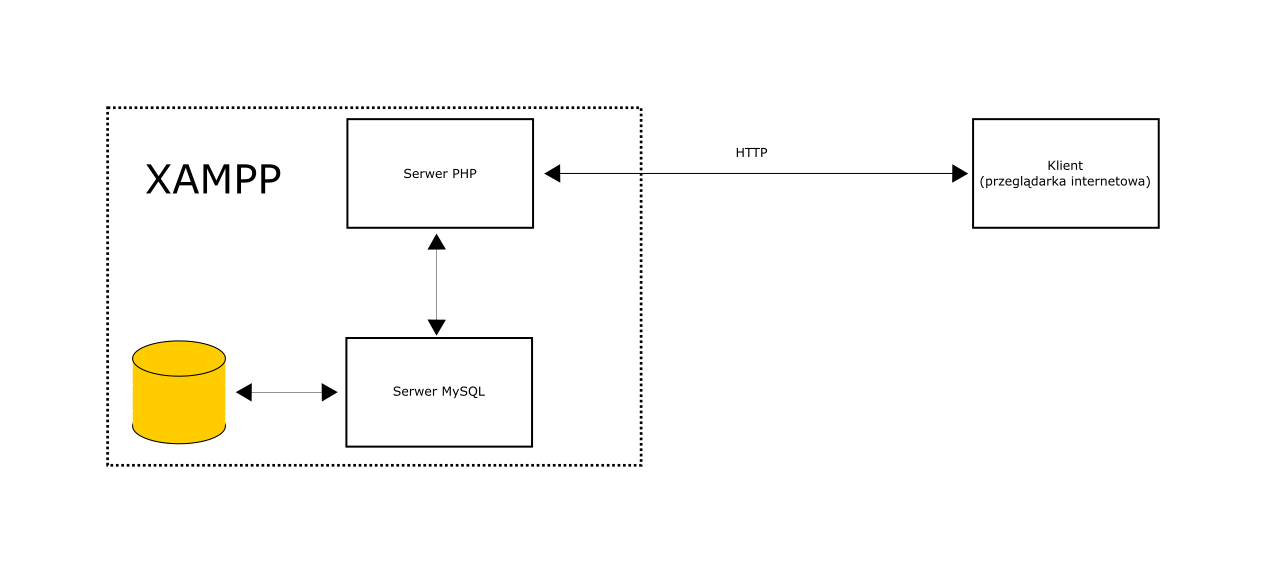
\includegraphics[height=7cm]{schemat.png}
	\caption[Schemat logiczny systemu]{Schemat logiczny systemu}
	\label{fig:schematLogiczny}
\end{figure}

\subsection{Wymagania funkcjonalne}
\subsubsection{Diagram przypadków użycia}
Funkcjonalności dla poszczególnych użytkowników systemu zebrano w~Tablicy~\ref{tab:tabelaPrzypadkowUzycia}.
Diagram przypadków użycia zamieszczony został na Rysunku~\ref{fig:diagramPrzypadkowUzycia}.

\begin{table}[H]
	\centering
	\caption[Tabela przypadków użycia]{Przypadki użycia dla poszczególnych użytkowników}
	\label{tab:tabelaPrzypadkowUzycia}
		\begin{tabular}{ l c c c c }
			Operacja/Użytkownik & Sprzedawca & Kierownik & Klient \\ \hline
			Zarządzanie kontami użytkowników & Tak & Nie & Nie \\ \hline
			Sprzedaż towaru & Tak & Nie & Nie \\ \hline
			Zarządzanie towarami w magazynie & Nie & Tak & Nie \\ \hline
			Zarządzanie sprzedawcami & Nie & Tak & Nie \\ \hline
			Przeglądanie raportów\\ sprzedaży & Nie & Tak & Nie \\ \hline
			Przeglądanie listy towarów & Nie & Nie & Tak \\ \hline
			Przeglądanie historii zakupów & Nie & Nie & Tak \\ \hline
			Zakup towarów & Nie & Nie & Tak \\ \hline
		\end{tabular}
\end{table}

\begin{figure}[H]
	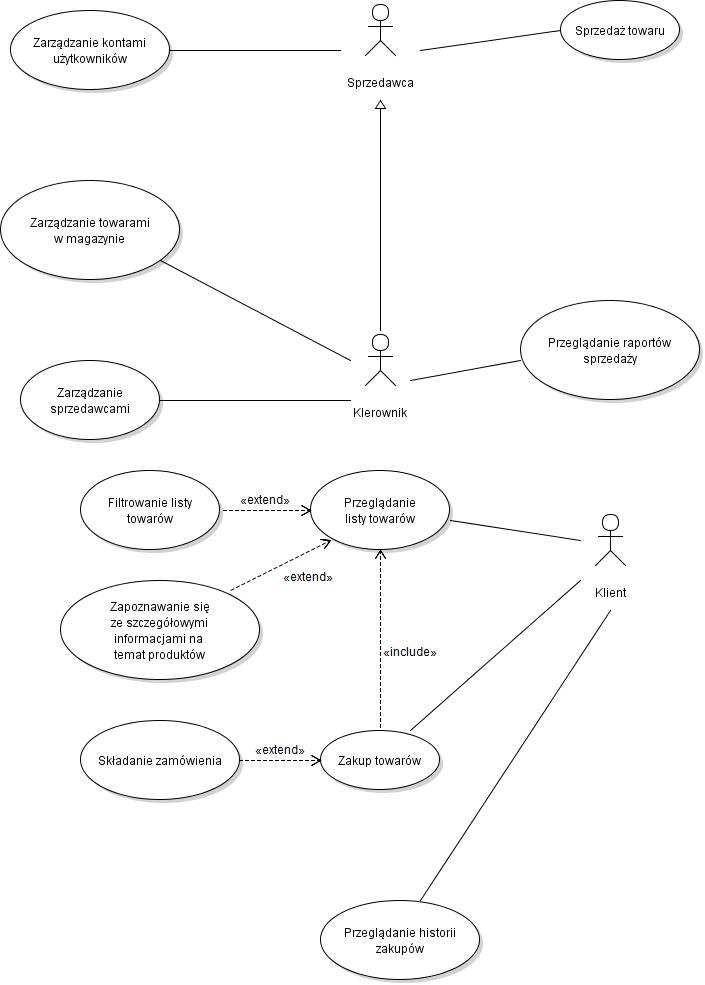
\includegraphics[width=13cm]{diagram_przypadkow_uzycia.jpg}
	\caption[Diagram przypadków użycia]{Diagram przypadków użycia}
	\label{fig:diagramPrzypadkowUzycia}
\end{figure}

\subsubsection{Scenariusze wybranych przypadków użycia}
\begin{itemize}
\item Filtrowanie listy dostępnych towarów
\begin{enumerate}
\item Użytkownik przegląda listę towarów.
\item Uzytkownik filtruje dostępne towary według producentów lub kategorii.
\item System wykonuje zapytanie o towary z podanym kryterium.
\item System przedstawia użytkownikowi znalezione towary.
\item Użytkownik dodaje wybrane produkty do zamówienia.
\end{enumerate}

\item Złożenie zamówienia
\begin{enumerate}
\item Użytkownik dodaje produkty do zamówienia.
\item Uzytkownik wybiera potwierdzenie zamówienia.
\item System realizuje zamówienie.
\item System powiadamia użytkownika o statusie operacji utworzenia zamówienia.
\end{enumerate}
\end{itemize}

\subsection{Wymagania niefunkcjonalne}
\subsubsection{Wykorzystywane technologie i narzędzia}
Technologie:
\begin{itemize}
	\item Implementacja systemu
	\begin{itemize}
		\item PHP 7.0
		\item MySQL 5.7.10
		\item HTML 5
		\item CSS 3
	\end{itemize}
	\item Testy funkcjonalne
	\begin{itemize}
		\item Java SE 8
		\item JDBC
		\item SeleniumHQ
	\end{itemize}
	\item Dokumentacja
	\begin{itemize}
		\item LaTeX
	\end{itemize}
\end{itemize}
Narzędzia projektowania:
\begin{itemize}
	\item MySQL 5.7.11
	\item MySQL Workbench 6.1
\end{itemize}
Narzędzia implementacji systemu:
\begin{itemize}
	\item GitHub Desktop 3.0.15
	\item NetBeans IDE 8.1
	\item XAMPP 5.6.19
\end{itemize}
\subsubsection{Wymagania dotyczące rozmiaru bazy danych}
Baza danych powinna przechowywać dane kilkuset artykułów sportowych wraz z~ich~aktualną ilością na~magazynach. Część danych związana z~administracją systemem w~stosunku do~ilości artykułów jest dużo mniejsza, w~związku z~czym~w~odniesieniu do~rozmiaru bazy danych została zaniedbana.
\subsubsection{Wymagania dotyczące bezpieczeństwa systemu}
\begin{itemize}
	\item System powinien być odporny na ataki typu SQL injection.
	\item Dostęp do bazy danych powinien odbywać~się poprzez uwierzytelnienie użytkownika.
	\item Każdy użytkownik powinien mieć dostęp do~danych, do~których wglądu jest uprawniony.
	\item Użytkownicy, którzy nie muszą modyfikować pozycji w tabelach, nie powinni otrzymywać do tego uprawnień ze~strony systemu.
\end{itemize}
\subsection{Przyjęte założenia projektowe}
System powinien być prosty w~obsłudze i~intuicyjny dla użytkownika, dodatkowo musi prawidłowo realizować swoje funkcjonalności i~prowadzić ciągły nadzór nad~danymi wprowadzanymi przez użytkownika a~także na~bieżąco informować o~wszelkich nieprawidłowościach. Czas przetwarzania dancyh oraz kierowanych zapytań nie~może~przekraczać kilku sekund.
\section{Projekt systemu}
\subsection{Projekt bazy danych}
\subsubsection{Analiza rzeczywistości i uproszczony model konceptualny}
\paragraph{Analiza rzeczywistości} \mbox{}\\
Sklep sportowy 'Sportpol' prowadzi sprzedaż detaliczną produktów sportowych na~rynku krajowym. Zadaniem sklepu~jest dostarczenie klientom szerokiego zakresu asortymentu oraz~możliwości wygodnego i~szybkiego dokonywania zakupów przez internet. Polityką firmy jest ciągłe zwiększanie sprzedaży wysyłkowej.

\paragraph{Model konceptualny} \mbox{}\\
Model konceptualny bazy danych przedstawiono na~Rysunku~\ref{fig:modelKonceptualny}.
\begin{figure}[H]
	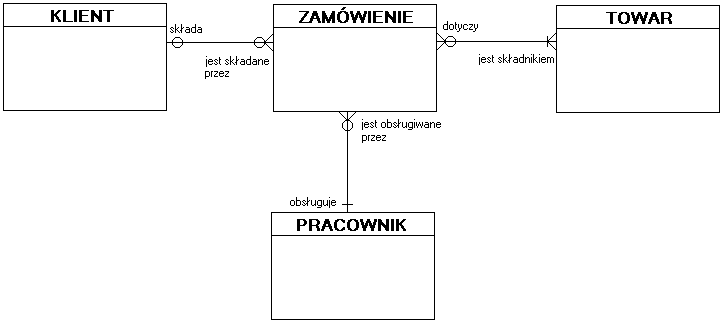
\includegraphics[width=14cm]{modelKonceptualny.png}
	\caption[Model konceptualny bazy danych]{Model konceptualny bazy danych}
	\label{fig:modelKonceptualny}
\end{figure}

\subsubsection{Model logiczny i normalizacja}
Model logiczny bazy danych zamieszczono na~Rysunku~\ref{fig:modelLogiczny}.
\begin{figure}[H]
	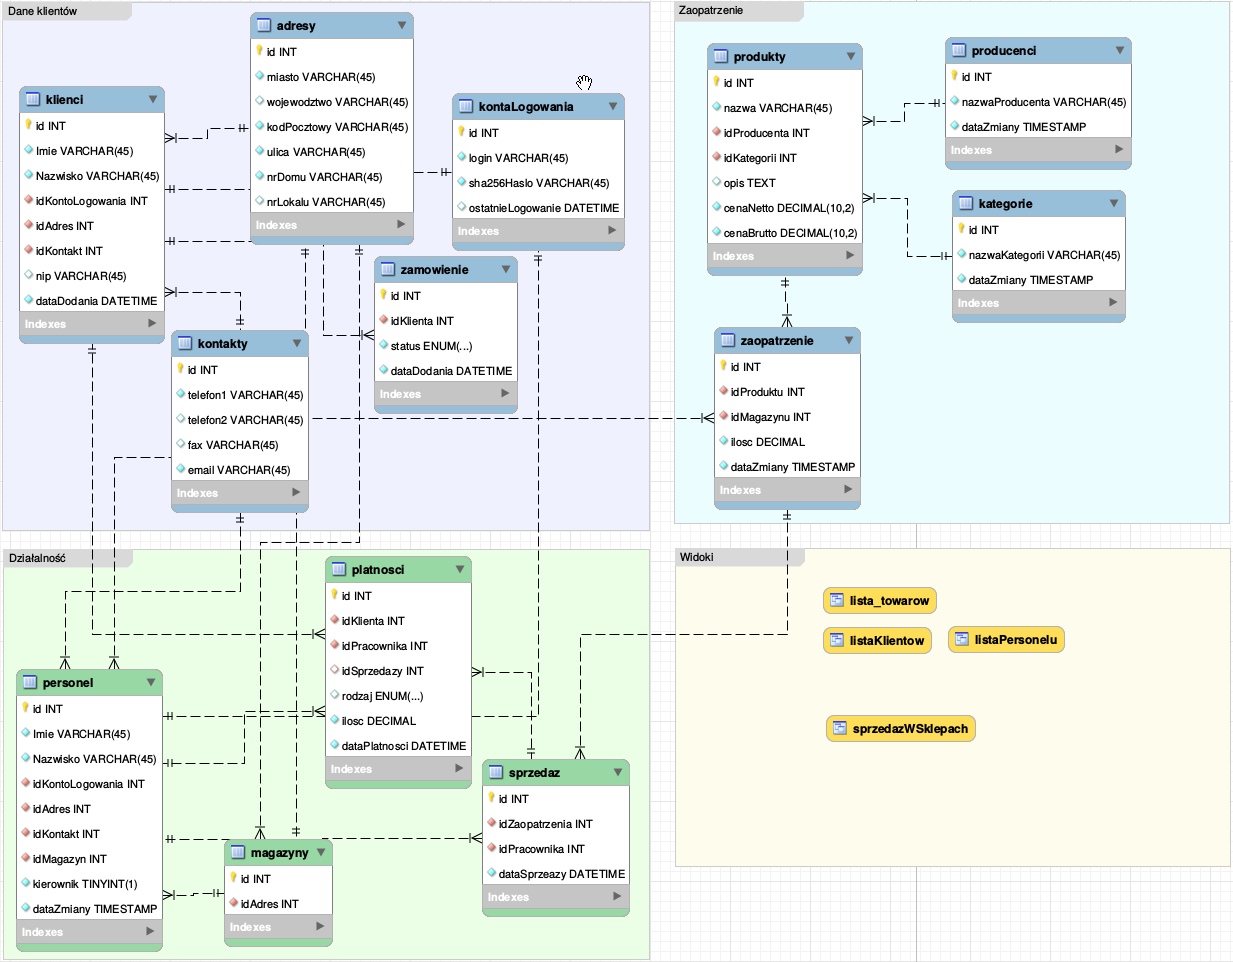
\includegraphics[width=14cm]{modelLogiczny.png}
	\caption[Model logiczny bazy danych]{Model logiczny bazy danych}
	\label{fig:modelLogiczny}
\end{figure}
\subsubsection{Model fizyczny i ograniczenia integralności danych}
\paragraph{Ograniczenia integralności danych} \mbox{}\\
Integralność i~spójność danych powinna być zapewniona triggery i procedury. Produkty dodawane do~zamówień powinny być jednocześnie odejmowane z~magazynów. W przypadku gdy zamówienie nie~może zostać zrealizowane, transakcja z~bazą danych powinna zostać wycofana i~nie~modyfikować stanu rekordów.

\paragraph{Model fizyczny} \mbox{}\\
Model fizyczny bazy danych zamieszczono na~Rysunku~\ref{fig:modelFizyczny}.
\begin{figure}[H]
	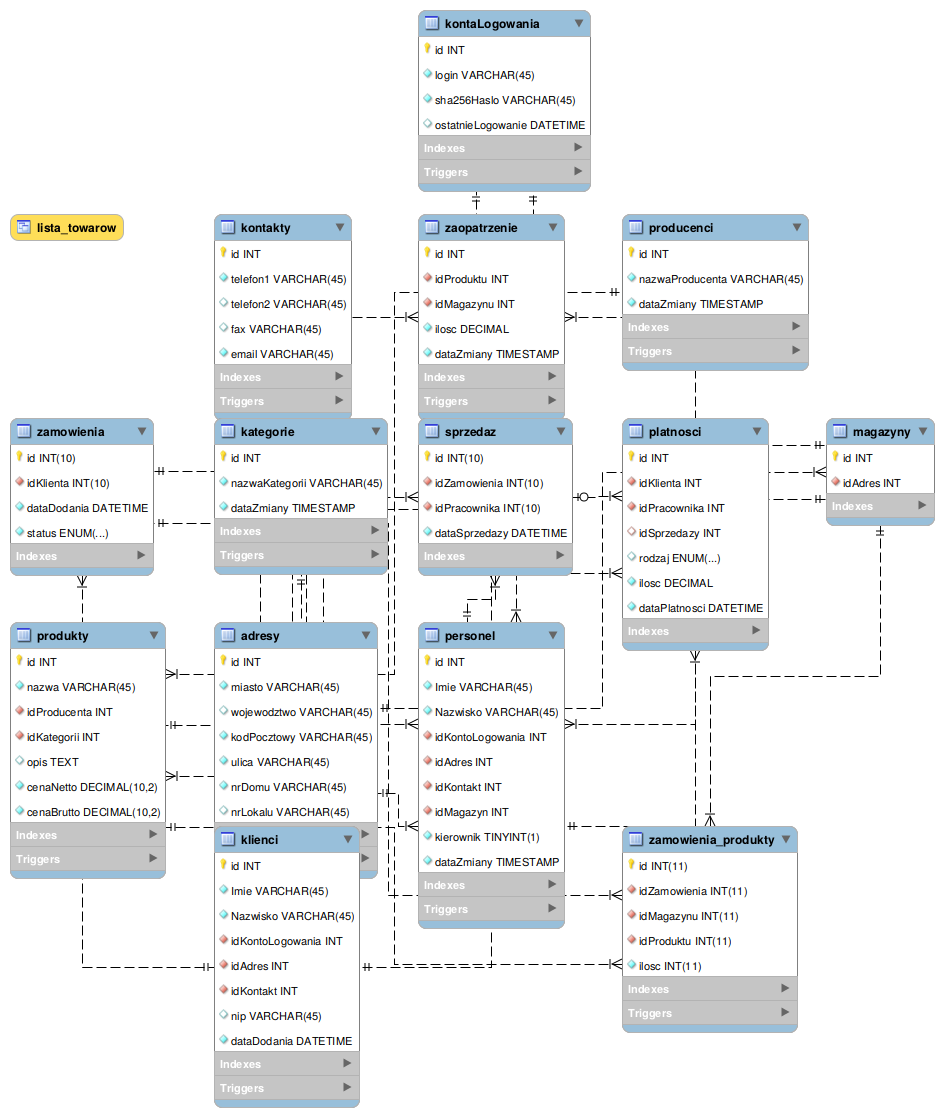
\includegraphics[width=14cm]{modelFizyczny.png}
	\caption[Model fizyczny bazy danych]{Model fizyczny bazy danych}
	\label{fig:modelFizyczny}
\end{figure}

\subsubsection{Inne elementy schematu – mechanizmy przetwarzania danych}
\begin{itemize}
\item Przetwarzanie danych powinno odbywać się w~większości przypadków po~stronie bazy danych
\item Użytkownik nie powinien uczestniczyć w~przetwarzaniu danych między systemem a~bazą danych
\item Wymiana dancyh powinna odbywać~się wyłącznie za~pomocą mechanizmów takich jak:
\begin{itemize}
\item Zapytania
\item Funkcje
\item Procedury
\item Widoki
\end{itemize}
\end{itemize}
\subsubsection{Projekt mechanizmów bezpieczeństwa na poziomie bazy danych}
Zabezpieczenia po~stronie bazy danych powinny sprowadzać się wyłącznie do~ograniczenia dostępu nieautoryzowanym użytkownikom oraz walidacji wprowadzanych danych za~pomocą wyrażej regularnych zaimplementowanych w~postaci triggerów. Inne sposoby ochrony danych nie~są~wymagane, ze~względu na~walidację po~stronie aplikacji dostępowej.
\subsection{Projekt aplikacji użytkownika}
\subsubsection{Architektura aplikacji i diagramy projektowe}
Aplikacja zbudowana jest w~oparciu o~część webową w~postaci strony internetowej \textit{HTML}, a~także serwerową napisaną za~pomocą języka \textit{PHP}. Schemat połączeń pomiędzy elementami aplikacji przedstawiono na~Rysunku~\ref{fig:architekturaAplikacji}.

\begin{figure}[H]
	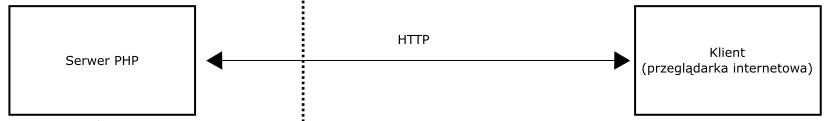
\includegraphics[width=14cm]{modelAplikacji.png}
	\caption[Architektura aplikacji]{Model architektoniczny aplikacji dostępowej}
	\label{fig:architekturaAplikacji}
\end{figure}

\subsubsection{Interfejs graficzny i struktura menu}
\subsubsection{Projekt wybranych funkcji systemu}
\begin{table}[H]
	\caption[Zestawienie wybranych funkcji systemu]{Zestawienie wybranych funkcji systemu}
	\label{tab:wybraneFunkcjeSystemu}
		\hskip-2.5cm\begin{tabular}{ l c c }
			Operacja & Dane wejściowe & Dane wyjściowe \\ \hline
			Przeglądanie produktów & Lista \textit{ID} producentów i lista \textit{ID} kategorii & Przefiltrowana tabela produktów \\ \hline
		    Tworzenie zamówienia & \textit{ID} klienta i lista towarów wraz z ilościami & Powodzenie operacji \\ \hline
		\end{tabular}
\end{table}

\subsubsection{Metoda podłączania do bazy danych – integracja z bazą danych}
Komunikacja z~bazą danych ze~strony serwerowej odbywa się za~pomocą biblioteki języka PHP, umożliwiającej wydawanie zapytań SQL.
\subsubsection{Projekt zabezpieczeń na poziomie aplikacji}
Wydawanie zapytań ze~strony aplikacji możliwe jest wyłącznie za~pomocą interfejsu dostępowego. Wszelkie operacje związane z~bazą danych są~ukryte poprzez interfejs użytkownika, w~związku z~czym nie~jest możlie uzyskanie dostępu do~danych w~sposób inny, niż ten oferowany przez aplikację.

\section{Implementacja systemu}
\subsection{Realizacja bazy danych}
\subsubsection{Tworzenie tabel i definiowanie ograniczeń}
\paragraph{Tworzenie tabel}
Inicjalizacja systemu bazodanowego odbywa~się za~pomocą usługi phpmyadmin. W~celu zalogowania do~usługi, należy wybrać w~przeglądarce internetowej adres \url{http://localhost/phpmyadmin} oraz wprowadzić dane logowania do~formularza przedstawionego na~Rysunku~\ref{fig:logowanieDophpMyAdmin}. Następnie należy wybrać z~menu opcję \textit{Import} (Rysunek \ref{fig:phpMyAdmin}), \textit{Import z pliku .sql}, podać ścieszkę do~przygotowanego pliku z~bazą danych i~zatwierdzić operację poprzez wybranie \textit{OK}.

\snippet{SQL}{tworzenieTabel.sql}

\paragraph{Definiowanie ograniczeń}
Ograniczenia dotyczące poprawności wprowadzanych danych przez użytkownika zaimplementowane są~w postaci \textit{triggerów}, które są~automatycznie ładowane do~bazy danych w~chwili importowania przygotowanego pliku \textit{.sql}.

\snippet{SQL}{triggery.sql}

\subsubsection{Implementacja mechanizmów przetwarzania danych}
Mechanizmy przetwarzania danych pomiędzy systemem bazodanowym a bazą danych zrealizowane są za pomocą \textit{procedur}, \textit{funkcji} oraz \textit{widoków}. Wybrane mechanizmy stosowane w systemie zestawiono poniżej:

\begin{enumerate}
\item Procedura - dodajDoZamowienia
\begin{itemize}
\item Dodaje do zamówienia wybrane towary.
\item Aktualizuje stan magazynów.
\item W przypadku wyczerpania zasobów na magazynie, usuwa rekord z tabeli.

\snippet{SQL}{procedura.sql}

\end{itemize}
\item Procedura - filtrujProdukty
\begin{itemize}
\item Przyjmuje listę \textit{ID} producentów i/lub kategorii.
\item Filtruje dane w tabeli produktów względem zadanych kryteriów.
\item Zwraca użytkownikowi wyłącznie dopasowane rekordy.
\end{itemize}
\item Funkcja - otwórzZamówienie
\begin{itemize}
\item Tworzy rekord w tabeli z zamówieniami.
\item Zwraca id utworzonego zamówienia.

\snippet{SQL}{funkcja.sql}

\end{itemize}
\item Widok - listaTowarów
\begin{itemize}
\item Dołącza do tabeli produktów
\begin{itemize}
\item Nazwy producentów
\item Nazwy kategorii
\item Informacje o stanie magazynów
\end{itemize}
\end{itemize}
\end{enumerate}

\subsubsection{Implementacja uprawnień i innych zabezpieczeń}
\paragraph{Dostęp do bazy danych} \mbox{}\\
Dostęp do bazy danych odbywa się za pośrednictwem usługi phpMyAdmin, świadczonej jako usługa webowa pod adresem \url{http://localhost/phpmyadmin} lub \url{http://127.0.0.1/phpmyadmin}. W celu uzyskania dostępu do~bazy danych, należy przejść przez procedurę uwieżytelnienia przedstawioną na~Rysunku~\ref{fig:logowanieDophpMyAdmin}.
\paragraph{Uwierzytelnianie w systemie} \mbox{}\\
Każdy użytkownik serwisu posiada własne konto w~systemie, wraz~z~przydzielonymi uprawnieniami do~wglądu bądź~modyfikacji danych.
Powyższa funkcjonalność pozwala ograniczyć przypadki ingerencji osób nieupoważnionych.\\\\
Serwis umożliwia także wygodną administrację dla użytkownika \textit{root}, co przedstawiono na~Rysunku~\ref{fig:phpMyAdmin}.

\begin{figure}[H]
	\centering
	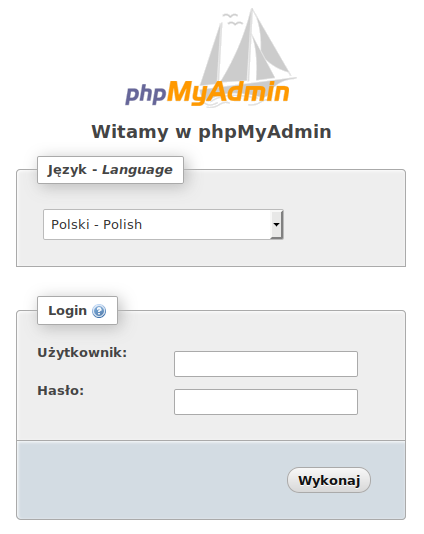
\includegraphics[width=9cm]{phpMyAdmin_login.png}
	\caption[Panel logowania do phpMyAdmin]{Panel logowania do usługi phpMyAdmin}
	\label{fig:logowanieDophpMyAdmin}
\end{figure}

\begin{figure}[H]
	\centering
	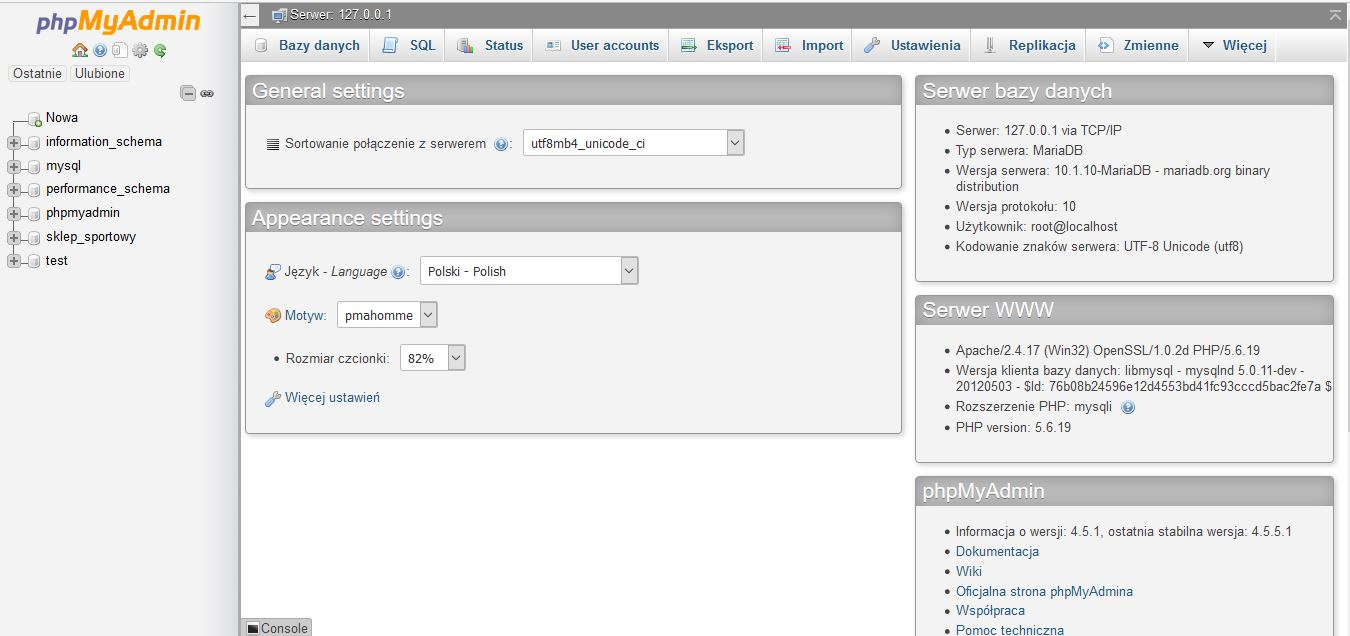
\includegraphics[width=15cm]{phpmyadmin.jpg}
	\caption[Panel administracyjny usługi phpMyAdmin]{Panel administracyjny usługi phpMyAdmin}
	\label{fig:phpMyAdmin}
\end{figure}
\subsection{Realizacja elementów aplikacji}
\subsubsection{Obsługa menu}
\subsubsection{Walidacja i filtracja}
System zapewnia walidację po stronie aplikacji jak i bazy danych. Uzupełnianie pól w aplikacji jest analizowane z poziomu interfejsu użytkownika oraz w przypadku nieprawidłowości, natychmiast kierowane są do użytkownika stosowne ostrzeżenia. Po stronie systemu bazodanowego, przed złożeniem zamówienia, sprawdzany jest stan produktów na magazynach. W przypadku niewystarczającej ilości towarów, zamówienie jest wycofywane z~systemu i~użytkownik otrzymuje powiadomienie o niepowodzeniu operacji.
\subsubsection{Implementacja interfejsu dostępu do bazy danych}
Dostęp do systemu odbywa się za pomocą interfejsu przedstawionego na~Rysunku~\ref{fig:interfejsUżytkownika}.

\begin{figure}[H]
	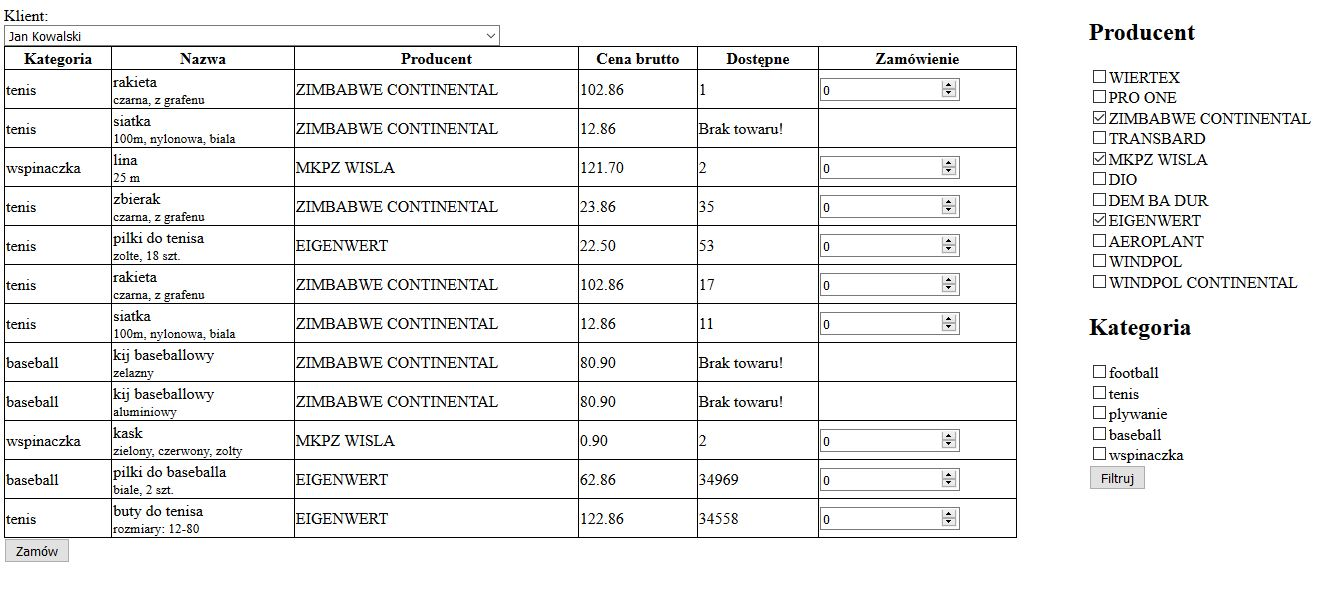
\includegraphics[width=14cm]{Screeny/Filtrowanie2.JPG}
	\caption[Interfejs użytkownika]{Interfejs użytkownika aplikacji dostępowej}
	\label{fig:interfejsUżytkownika}
\end{figure}

Użytkownik ma możliwość wyboru z listy rozwijanej (Rysunek~\ref{fig:listaRozwijana}) nazwy konta na które będzie realizowane zamówienie. Dodatkowo istnieje możliwość filtrowania listy aktualnie wyświetlonych produktów za pomocą panelu znajdującego się na~Rysunku~\ref{fig:panelFiltrowaniaProduktów}.

\begin{figure}[H]
	\centering
	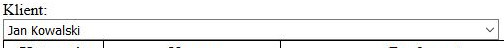
\includegraphics[width=10cm]{Screeny/listaRozwijana.JPG}
	\caption[Lista wyboru użytkownika]{Lista wyboru użytkownika składającego zamówienie}
	\label{fig:listaRozwijana}
	
	\centering
	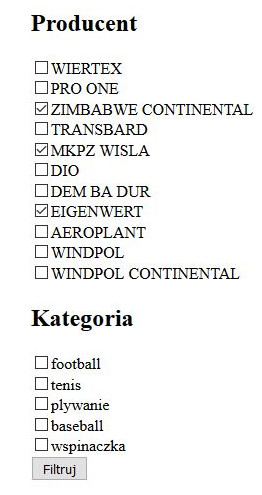
\includegraphics[height=10cm]{Screeny/panelFiltrowania.JPG}
	\caption[Panel filtorwania dostępnych produktów]{Panel filtorwania dostępnych produktów}
	\label{fig:panelFiltrowaniaProduktów}
\end{figure}

\subsubsection{Implementacja wybranych funkcjonalności systemu}
\paragraph{Przeglądanie listy towarów} \mbox{}\\
System wykonuje zapytanie do bazy danych o zestawienie danych dotyczących produktów wraz z podaniem aktualnego stanu ze wszystkich magazynów. Dodatkowo, jeżeli użytkownik poda listę producentów bądź listę kategorii, wywoływana jest procedura \textit{filtrujProdukty}, za pomocą której wydobywane są dane spełniające zadane kryteria. Dane są zwracane jako widok listaTowarów.
\paragraph{Tworzenie zamówienia} \mbox{}\\
Po wybraniu przez klienta wybranych produktów i naciśnięciu przycisku \textit{Zamów} tworzone jest zamówienie za pomocą funkcji otworzZamowienie. Następnie wybrane przez klienta pozycje są dodawna do zamówienia za pomocą procedury \textit{dodajDoZamowienia}. Po uzupełnieniu danych transakcja kierowana jest do bazy danych, gdzie przed wstawieniem każdego rekordu przechodzi przez proces walidacji. Sprawdzana jest poprawność semantyczna wprowadzonych rekordów oraz logiczna w postaci porównania ilości towarów ze stanem na magazynach. W rezultacie zwracane jest \textit{ID} utworzonego zamówienia. W przypdaku niepowodzenia, transakcja jest wycofywana z systemu. Możliwy stan operacji przedstawiono na~Rysunkach~\ref{fig:stanZamówieniaPowodzenie}~oraz~\ref{fig:stanZamówieniaNiepowodzenie}.

\begin{figure}[H]
	\centering
	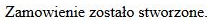
\includegraphics[width=7cm]{Screeny/ZamowieniePoprawne.JPG}
	\caption[Stan zamówienia - powodzenie operacji]{Komunikat o stanie utworzonego zamówienia - powodzenie operacji}
	\label{fig:stanZamówieniaPowodzenie}

	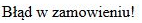
\includegraphics[width=5cm]{Screeny/ZamowienieNiepoprawne.JPG}
	\caption[Stan zamówienia - niepowodzenie operacji]{Komunikat o stanie utworzonego zamówienia - niepowodzenie operacji}
	\label{fig:stanZamówieniaNiepowodzenie}
\end{figure}
\paragraph{Filtrowanie produktów} \mbox{}\\
Podczas przeglądania tabeli dostępnych produktów użytkownik może dokonać filtracji poprzez wybranie w panelu bocznym z~Rysunku~\ref{fig:panelFiltrowaniaProduktów} producentów bądź kategorii. Po naciśnięciu przycisku \textit{Filtruj} wywoływana jest procedura \textit{filtrujProdukty} zwracająca widok. Następnie dane są wyświetlane użytkownikowi. Przykładowy wynik operacji zamieszczono na~Rysunku~\ref{fig:rezultatFiltracji}.

\begin{figure}[H]
	\centering
	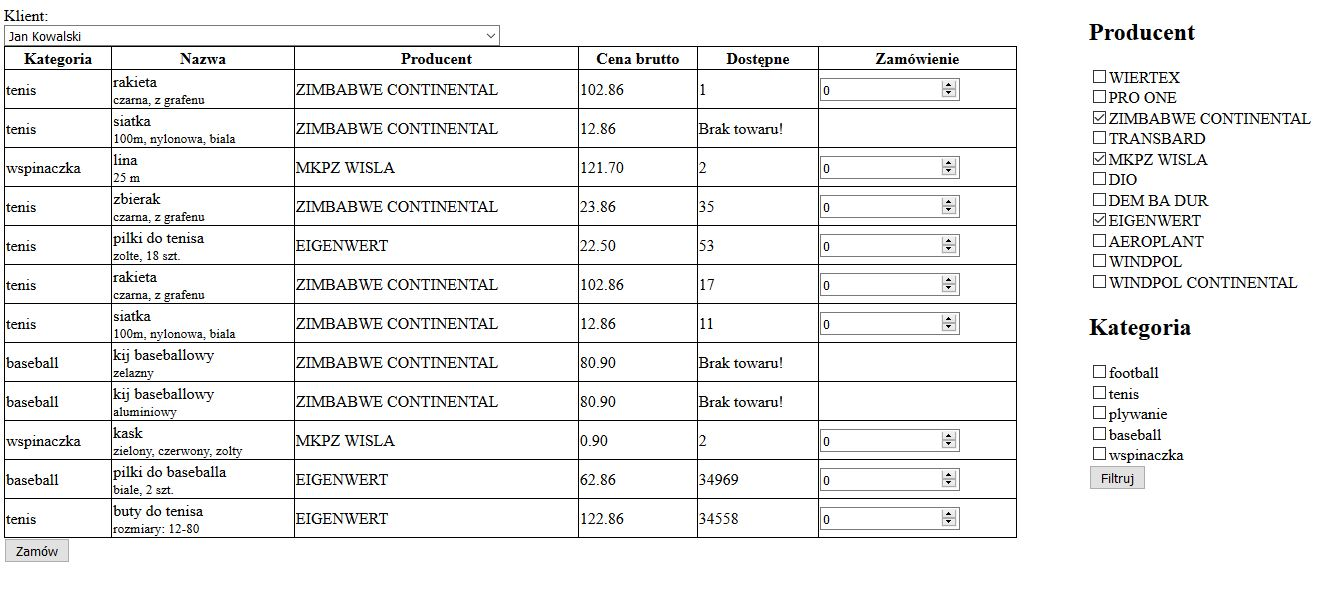
\includegraphics[width=14cm]{Screeny/Filtrowanie2.JPG}
	\caption[Widok tabeli towarów po filtracji]{Widok tabeli towarów po filtracji}
	\label{fig:rezultatFiltracji}
\end{figure}

\subsubsection{Implementacja mechanizmów bezpieczeństwa}
\paragraph{Sprawdzanie stanu magazynów} \mbox{}\\
Mechanizmy bezpieczeństwa systemu opierają się o~sprawdzenie ilości stanu danych na~magazynie, co~sprowadza się do~kierowania zapytań do~bazy danych o~aktualny stan towarów i~uniemożliwienie użytkownikowi wybrania większej ilości niż jest dostępne.
\paragraph{Triggery} \mbox{}\\
Dodatkowym zaimplementowanym mechanizmem są trigery pozwalające na walidację rekordów bazy poprzez zastosowanie wyrażeń regularnych. W systemie są wykorzystywane podczas wstawiania rekordów do tabel, w przypadku niezgodności z wyrażeniem rekord jest odrzucany. Wybrane triggery zaimplementowane w~systemie zestawiono w~Tablicy~\ref{tab:tabelaTrigerów}.

\begin{table}[H]
	\caption[Tablica wybranych triggerów]{Tablica wybranych triggerów zaimplementowanych w systemie}
	\label{tab:tabelaTrigerów}
		\hskip-1cm\begin{tabular}{ l l }
			Trigger & Wyrażenie regularne \\ \hline
			Kod pocztowy & \verb=^[0-9]{2}\-[0-9]{3}= \\ \hline
			Ulica & \verb=^((ul.|al.|os.|rondo|zaułek|skwer)\ )([A-Za-z]{2,100}\ ?)+= \\ \hline
			NIP & \verb=^[0-9]{10}|[0-9]{3}\-[0-9]{3}\-[0-9]{2}\-[0-9]{2}= \\ \hline
			Telefon & \verb=^(\\+?[0-9]{1,4}-?)?[0-9]{3,10}= \\ \hline
			Nazwa producenta & \verb=^([A-Za-z0-9]{2,100}\ ?){1,100}= \\ \hline
			Hasło sha256 & \verb=^[0-9a-f]{32}= \\ \hline
		\end{tabular}
\end{table}


\section{Testowanie systemu}
\subsection{Instalacja i konfigurowanie systemu}
\paragraph{Do pobrania}
\begin{enumerate}
	\item XAMPP - \url{https://www.apachefriends.org/pl/index.html}
	\item GitHub - \url{https://desktop.github.com/}
	\item NetBeans \textbf{dla PHP} - {\url{https://netbeans.org/downloads/}}
\end{enumerate}
\paragraph{XAMPP}
\begin{enumerate}
	\item Zainstaluj XAMPP`a
	\item Otwórz \quotedblbase XAMPP Control Panel\textquotedblright
	\item W linijce \quotedblbase Apache\textquotedblright wybierz \quotedblbase Start\textquotedblright
	\item Wejdź do przeglądarki internetowej
	\item Wejdź na \url{http://localhost} (ewentualnie \url{http://localhost:80}). Jeżeli zobaczyłeś stronę internetową, to znaczy, że się udało.
\end{enumerate}
\paragraph{Github}
\begin{enumerate}
	\item Pobierz projekt z repozytorim \url{https://github.com/shortname/dazybanych/archive/master.zip}
	\item Rozpakuj pobrane archiwum w wybranej lokalizacji.
	\item Znajdź w folderze, gdzie zainstalowałeś XAMPP`a plik apache/conf/extra/httpd-vhosts.conf
	\item Dopisz na końcu znalezionego pliku tekst \lstinputlisting{wklejka.txt}, zamieniając XXX na ścieżkę do katalogu z pobranym projektem.
	\item Uruchom serwer \quotedblbase Apache\textquotedblright z poziomu \quotedblbase XAMPP Control Panel\textquotedblright
	\item Wejdź do przeglądarki internetowej
	\item Wejdź na \url{http://localhost}. Jeżeli zobaczyłeś stronę \quotedblbase Hello world!\textquotedblright, to znaczy, że operacja powiodła się
\end{enumerate}
\paragraph{MySql Server}
\begin{enumerate}
	\item Zainstaluj XAMPP.
	\item Otwórz \quotedblbase XAMPP Control Panel\textquotedblright
	\item W linijkach \quotedblbase Apache\textquotedblright , \quotedblbase MySQL\textquotedblright wybierz \quotedblbase Start\textquotedblright
	\item Otwórz przeglądarkę internetową i wejdź na \url{http://localhost/phpmyadmin} i sprwadź czy pojawiło się okno logowania z Rysunku \ref{fig:logowanieDophpMyAdmin}.
	\item Wejdź w zakładkę \quotedblbase User accounts\textquotedblright, zaznacz wszystkich użytkowników poza \quotedblbase root\textquotedblright na \quotedblbase localhost\textquotedblright i kliknij \quotedblbase Wykonaj\textquotedblright u dołu strony.
	\item W ustawieniach zmień hasło na \quotedblbase admin\textquotedblright i kliknij \quotedblbase Wykonaj\textquotedblright.
	Po odświeżeniu strony powinien pokazać się następujący komunikat:
	\texttt{\quotedblbase Nie udało się nawiązać połączenia: błędne ustawienia.\textquotedblright}.
	\item Znajdź w folderze instalacyjnym XAMPP`a plik phpMyAdmin/config.inc.php
	\item W znalezionym pliku zmień wartość przypisania:\\
			\begin{lstlisting}
$cfg['Servers'][$i]['password'] = '';
			\end{lstlisting}
			na 'admin'
		\item Po odświeżeniu strony powinienieś zobaczyć panel administracyjny bazy danych.
		\item Z górnego menu wybierz \quotedblbase Import\textquotedblright. W widoku importu wybierz plik z Baza Danych/sklep{\_}sportowy.sql, upewnij się, że ustawione jest kodowanie znaków jako \quotedblbase utf-8\textquotedblright. Kliknij \quotedblbase Wykonaj\textquotedblright.
		\item Otwórz przeglądarkę i wejdź na \url{http://localhost/login.php}
		\item Po zalogowaniu (\quotedblbase admin\textquotedblright, \quotedblbase admin\textquotedblright) powinna wyświetlić się lista towarów. Wszystkie polskie znaki powinny być wyświetlane poprawnie.
\end{enumerate}

\subsection{Testowanie opracowanych funkcji systemu}
Testowanie funkcjonalności odbywało się za~pomocą środowiska \textit{Selenium}, dzięki któremu można było symulować zachowanie użytkownika naciskającego kolejne elementy interfejsu dostępowego. Dodatkowo do~komunikacji z~bazą danych wykorzystano framework \textit{JDBC}, za~pomocą którego kierowane były zapytania do~bazy danych z~języka \textit{JAVA}. Przed przeprowadzeniem każdego testu baza danych była ładowana od~nowa, w~celu uniknięcia nieprawidłowości po~poprzednich testach.

\subsubsection{Testowanie zamówienia}
\paragraph{Zależności do sprawdzenia}
\begin{itemize}
\item Modyfikacje wprowadzane przez użytkownika modyfikują bazę danych.
\item Wielu użytkowników może wykonywać zamówienia bez kolizji.
\item Zamówienie jest zapisywane w bazie danych.
\item Stan magazynów jest aktualizowany po złożeniu każdego z zamówień.
\item Ilość produktów w zamówieniu odzwierciedla ilość podaną przez użytkownika.
\item Wszystkie zamówione produkty znajdują się w zamówieniu.
\end{itemize}

\paragraph{Przebieg testu}
\begin{enumerate}
\item Zresetowanie bazy do stanu wyjściowego.
\item Pobranie rekordów dotyczących modyfikowanych produktów z tabeli zaopatrzenie.
\item Zasymulowanie zmian na podanych rekordach oraz na tabelach `zamowienia` i `zamowienia\_produkty`.
\item Wejście na stronę z listą towarów.
\item Wyklikanie pierwszego zamówienia (ustawienie klienta, wpisanie ilości produktów).
\item Wejście na stronę z listą towarów.
\item Zasymulowanie zmian na podanych rekordach oraz na tabelach `zamowienia` i `zamowienia\_produkty`.
\item Porównanie stanu bazy danych przed i po transakcji.
\end{enumerate}
\subsubsection{Testowanie filtrowania}
\paragraph{Zależności do sprawdzenia}
\begin{itemize}
\item Kategorie oraz producenci zostali przypisani prawidłowo.
\item Suma ilości artykułów z magazynów jest prawidłowa.
\item Bez filtrowania wyświetlają się wszystkie produkty.
\item Przy podaniu kryteriów wynik działania obu będzie uwzględniony.
\end{itemize}
\paragraph{Przebieg testu}
\begin{enumerate}
\item Stworzenie zamówienia dla dwóch różnych klientów.
\item Sprawdzenie czy dane z tabel zamówienia, zamówienia\_produkty oraz zaopatrzenie zostały zmodyfikowane.
\end{enumerate}
\subsection{Testowanie mechanizmów bezpieczeństwa}
Zabezpieczenia interfejsu użytkownika przed niepoprawnym formatem danych zostały sprawdzone pod kątem przekroczenia stanu towarów na magazynie oraz poprawnej sygnalizacji błędów ze strony aplikacji. Rezultat testu przedstawiono na~Rysunku~\ref{fig:walidacja1} i~\ref{fig:walidacja2}.

\begin{figure}[H]
	\centering
	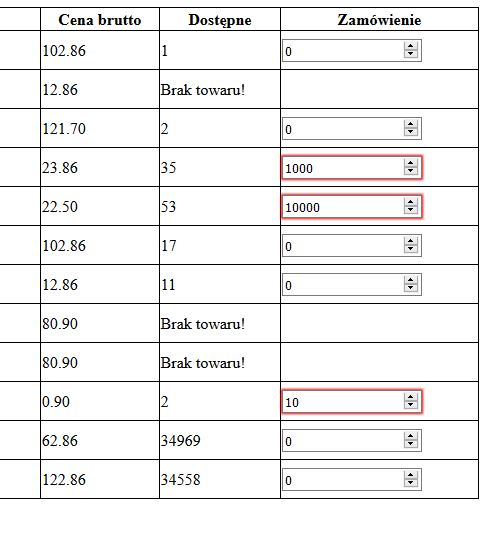
\includegraphics[height=9cm]{Screeny/Walidacja1.JPG}
	\caption[Walidacja danych po stronie aplikacji]{Walidacja danych po stronie aplikacji}
	\label{fig:walidacja1}

	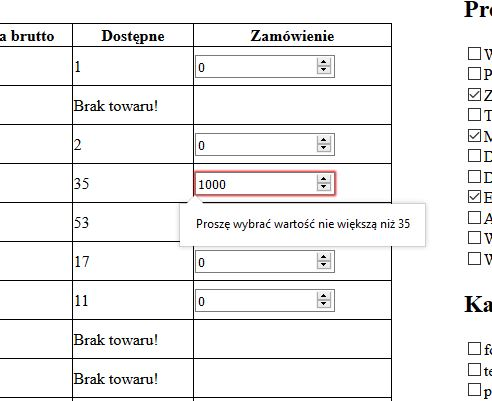
\includegraphics[height=9cm]{Screeny/Walidacja2.JPG}
	\caption[Walidacja danych po stronie aplikacji z komunikatem]{Walidacja danych po stronie aplikacji z komunikatem}
	\label{fig:walidacja2}
\end{figure}

Sprawdzono także odporność bazy danych na~nieporawny format danych w~przypadku błędu ze~strony aplikacji dostępowej. W~tym celu podjęta została próba ręcznego wprowadzenia danych w~formacie niezgodnym ze~specyfikacją. Rezultat powyższej operacji przedstawiony został na~Rysunku~\ref{fig:testTriggera}.
\begin{figure}[H]
	\centering
	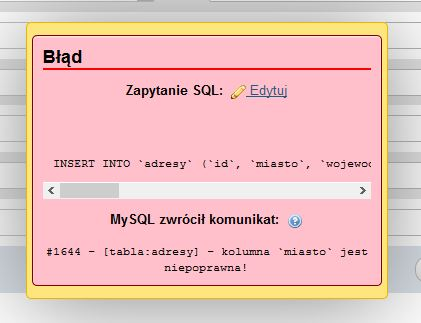
\includegraphics[height=7cm]{Screeny/TriggerDziala.JPG}
	\caption[Rezultat testu triggera]{Komunikat informujący o nieprawidłowym formacie danych}
	\label{fig:testTriggera}
\end{figure}
Weryfikacja odporności bazy danych na~ataki SQL Injection nie~była konieczna, ze~względu na~zabezpieczenie bazy danych przed nieupoważnionymi użytkownikami oraz ukryciem istnienia bazy danych przed klientem. Wszystkie zapytania obsługiwane są~za~pomocą aplikacji dostępowej, użytkownik nie~ma~możliwości wykonania zapytania bez~pośrednictwa systemu.
\subsection{Wnioski z testów}
Testy zweryfikowały poprawność działania zaimplementowanych funkcjonalności. Ich różnorodność pozwoliła na~sprawdzenie systemu na~różnych poziomach abstrakcji. Zastosowanie testów sprawdzających działanie interfejsu poprzez symulowanie zachowania użytkownika pozwoliło na~sprawdzenie systemu w~środowisku jak~najbardziej zbliżonym do~rzeczywistego użytkowania. Wszystkie testy zwróciły wynik pozytywny.
\section{Podsumowanie}
%Celem zadania było zaprojektowanie i zaimplementowanie relacyjnej bazy danych na potrzeby internetowego sklepu sportowego.
%Pierwszym krokiem było określenie przypadków użycia projektowanej aplikacji, które zebrano w formie diagramu. Kolejnym etapem fazy projektowej było stworzenie modelu konceptualnego, który obrazował relacje zachodzące pomiędzy zaplanowanymi tabelami. Gdy te zależności zostały określone,  
\begin{itemize}
	\item Cel projektu: zaprojektowanie i implementacja relacyjnej bazy danych na potrzeby sportowego sklepu internetowego; stworzenie prostej webowej aplikacji do obsługi wybranych funkcjonalności; przetestowanie funkcjonalności
	\item Kroki:
		\begin{itemize}
		\item Analiza rzeczywistości - zebranie wymagań funkcjonalnych i niefunkcjonalnych (funkcjonalnych w formie diagramu przypadków użycia)		
		\item Stworzenie diagramu konceptualnego - określenie jakie tabele będą potrzebne i jakie relacje między nimi zachodzą
		\item Diagram logiczny - co w tych tabelach będzie
		\item Diagram fizyczny - jakie typy bazodanowe są potrzebne, normalizacja(?)
		\item Dobór narzędzi i technologii
		\item Stworzenie tabel
		\item Stworzenie relacji pomiędzy tabelami (klucze obce)
		\item Triggery - walidacja danych wchodzących do bazy
		\item Widok
		\item Porcedury i funkcja - wykorzystanie wszystkich możliwości bazy danych (odciążenie back-endu)
		\item Aplikacja webowa - pokazanie, że stworzona baza może być praktycznie wykorzystana
		\item Testy funkcjonalne - sprawdzenie, czy mechanizmy bazodanowe funkcjonują poprawnie; ułatwienia dalszego rozwoju aplikacji
\end{itemize}		  
\end{itemize}
\cleardoublepage
\bibliographystyle {IEEEtran}
\bibliography {bibliografia}
\nocite {*}

\end{document}